%%%%%%%%%%%%%%%%%%%%%%%%%%%%%%%%%%%%%%%%%%%%%%%%%%%%%%%%%%%%%%%%%%%%%%%%%%%%%%%%%%%%%%%%
%
%  TeX template file for Journal of Evolving Space Activities (JESA)
%
%                 Ver.1.2  February 2023, ISTS Publication Committee
%%%%%%%%%%%%%%%%%%%%%%%%%%%%%%%%%%%%%%%%%%%%%%%%%%%%%%%%%%%%%%%%%%%%%%%%%%%%%%%%%%%%%%%%

%%%%%%%%%%%%%%%%%%%%%%%%%%%%%%
%---Only For Editors---
%%%%%%%%%%%%%%%%%%%%%%%%%%%%%%
\documentclass[JESA]{tjsass} % for JESA submission and peer review process
%\documentclass[JESA, pubform, CCBY]{tjsass} % for JESA publication by CCBY license
%\documentclass[JESA, pubform, CCBYNCND]{tjsass} % for JESA publication by CC-BY-NC-ND license

%%%%%%%%%%%%%%%%%%%%%%%%%%%%%%
%---Required Packages---
%%%%%%%%%%%%%%%%%%%%%%%%%%%%%%
%The packages below should be installed on your PC
\usepackage{graphicx}
\usepackage{subcaption}
\usepackage{appendix}
%\usepackage[dvipdfmx]{graphicx}
\usepackage{graphicx}
\RequirePackage{multicol}
\RequirePackage{amsmath}
\RequirePackage[varg]{txfonts}
\RequirePackage{bm}
\RequirePackage{array}
%\RequirePackage{color}
\RequirePackage{tjsasscite}
\usepackage[hang]{footmisc}
\newcommand{\bhline}[1]{\noalign{\hrule height #1}}

%%%%%%%%%%%%%%%%%%%%%%%%%%%%%%
%---Publication Info. Only For Editors---
%%%%%%%%%%%%%%%%%%%%%%%%%%%%%%
\pubyear{2024}% year of publication
\bookvolume{2}% volume
\articlenumber{140}% dummy article number which will be modified by editors
\setcounter{page}{1}% starting page number
\titleheadertrue% title for header
\receiveddate{August 31st, 2023}% dummy date which will be modified by editors

%%%%%%%%%%%%%%%%%%%%%%%%%%%%%%
%---Set up Title & Author---
%%%%%%%%%%%%%%%%%%%%%%%%%%%%%%

\title{Heteroclinic Connections Between Invariant Tori of Different Dimensions}% paper title
\subtitle{}% paper subtitle only when necessary
%
%%%%%% put author's name in \author{} following the rules below.
%%  \NAME{first name}{last name}   %last name is converted to capital letters.
%%  \thanksNum{affiliation}
%
\author{\NAME{Soichiro}{Shin}\thanksNum{1)}, 
        \NAME{Shanshan}{Pan}\thanksNum{1)}, 
        \NAME{Mai}{Bando}\thanksNum{1)}, 
        \NAME{Shinji}{Hokamoto}\thanksNum{1)}}
\CorresAuthor{shin.soichiro.103@s.kyushu-u.ac.jp}
%
%%%%%% \thanksOrg{}
%%%%%%   affiliations are automatically numbered.
%
% \thanksOrg{Institute of Space and Astronautical Science, JAXA, Sagamihara, Japan}% affiliation 1
\thanksOrg{Department of Aeronautics and Astronautics, Kyushu University, Fukuoka, Japan}% affiliation 1
%
%%%%%%%%%%%%%%%%%%%%%%%%%%%%%%
%---Abstract and Keywords---
%%%%%%%%%%%%%%%%%%%%%%%%%%%%%%
%
\begin{abstract}
This study investigates heteroclinic connections between orbits of different geometric dimensions in the Earth-Moon Circular Restricted Three-Body Problem(CR3BP). By examining various combinations of orbits with different geometric dimensions, this study evaluates the feasibility of manifold intersections. The dimensional analysis reveals that heteroclinic connections are generally realizable when the manifolds of a periodic orbit propagated along two eigenvector directions intersect with those of a quasi-periodic torus. Based on this result, numerical computations are conducted to propagate invariant manifolds and detect their intersections using a Poincaré seciton. The quasi-periodic orbits are computed via the GMOS algorithm, which constructs two-dimensional invariant tori through interpolation on a phase-space grid. Trajectories approximating heteroclinic connections are successfully obtained, highlighting the potential for low-energy orbit transitions between orbits of different topological structures. The findings contribute to the broader applicability of manifold-based trajectory design in future space mission planning.
\end{abstract}
%
\keywords{Heteroclinc Connection, Circular Restricted Three-Body Problem, Invariant Tori}
%
%%%%%%%%%%%%%%%%%%%%%%%%%%%%%%
%---Main Document Start---
%%%%%%%%%%%%%%%%%%%%%%%%%%%%%%
%
\begin{document}
\maketitle

\section*{Nomenclature}

\vbox{\noindent\setlength{\tabcolsep}{0mm}%
\begin{tabular}{p{25mm}cl} %
\hfil$x,y,z$\hfil & :\hspace{4mm} & Position coordinates \\
\hfil$\dot{x},\dot{y},\dot{z}$\hfil & :\hspace{4mm} & Velocity components \\
\hfil$\mu$\hfil & :\hspace{4mm} & Mass ratio of the two primaries  \\
\hfil$C$\hfil & :\hspace{4mm} & Jacobi constant \\
\hfil$L_1,L_2$\hfil & :\hspace{4mm} & First and second Lagrange points  \\
\hfil$\phi$\hfil & :\hspace{4mm} & State vector \\
\hfil$M$\hfil & :\hspace{4mm} & Monodromy matrix \\
\hfil$\lambda$\hfil & :\hspace{4mm} & Eigenvalue of the monodromy matrix \\
\hfil$W^s, W^u$\hfil & :\hspace{4mm} & Stable and unstable manifolds\\
\hfil$\mathcal{O}$\hfil & :\hspace{4mm} & An orbit in the phase space  \\
\hfil$t$\hfil & :\hspace{4mm} & Time variable
\end{tabular}}

\noindent{Subscripts}

\vbox{\noindent\setlength{\tabcolsep}{0mm}%
\begin{tabular}{p{25mm}cl}
\hfil$0$\hfil & :\hspace{4mm} & initial \\
\hfil$\mathrm{f}$\hfil & :\hspace{4mm} & final
\end{tabular}}

\section{Introduction}

In recent years, the resurgence of space exploration has revitalized interest in dynamical system theory, particularly the three-body problem. Among its formulations, the Circular Restricted Three-Body Problem(CR3BP) - in which the mass of one body is assumed to be negligible - has become a fundamental tool for spacecraft trajectory design under the influence of two primary celestial bodies.\cite{barrowgreen1997,szebehely1967} 

The CR3BP features five equilibrium points, known as Lagrange points. Orbits around $L_1$ and $L_2$ are particularly important in mission planning. For instance, NASA's Artemis program leverages these regions to ensure efficient and stable operations in the Earth-Moon system.

A key advantage of the CR3BP is its rich manifold structure. Invariant manifolds associated with periodic or quasi-periodic orbits enable low-energy transfers by following the natural dynamical flow. This manifold-based approach has been utilized in a wide variety of mission designs and theoretical studies.\cite{anderson2009,sanchez2016,kakoi2014,cox2021,dellnitz2006,moore2012,villegaspinto2021} A prominent application is NASA's Genesis mission, which successfully collected solar wind particles by exploiting the invariant manifold structure near the Sun-Earth $L_1$ point, thereby minimizing fuel consumption.\cite{koon2000}

Among manifold-based transfers, \textit{heteroclinic connections} - defined by the intersections between stable and unstable manifolds of distinct orbits - enables thrustless transfers and is particularly useful for cargo transport or recovery operations during anomalies.\cite{koon2000,henry2024,owen2024,olikara2016}

Recent research has extended the concept of heteroclinic connections to include quasi-periodic orbits, which exhibit multi-frequency recurrence and offer more flexible spatial coverage. Henry and Sheeres\cite{henry2024} developed a fully numerical method based on boundary value formulations, while Owen and Baresi\cite{owen2024} proposed a topological detection method using knot theory.

However, most existing studies have focused on heteroclinic connections between invariant sets of the same dimension, such as 1D-to-1D or 2D-to-2D transitions. Little attention has been paid to connections between orbits of different geometric dimensions, despite their potential to expand the design space of low-energy trajectories. A typical example is a transition between a one-dimensional Lyapunov orbit and a two-dimensional quasi-periodic torus.

This study addresses this gap by investigating heteroclinic connections between orbits of different dimensions in the Earth-Moon CR3BP. We first evaluate the dimensional conditions necessary for manifold intersection through dimensional analysis. Then, we numerically compute potential connections, visualize the resulting trajectories, and analyze their dynamical properties. This work aim to broaden the applicability of manifold-based design methodologies and contribute to future mission planning. 

\section{Background}

\subsection{Circular restricted three-body problem}

The Circular Restricted Three-Body Problem (CR3BP) describes the motion of a massless third body (e.g., a spacecraft) under the gravitational influence of two massive bodies: the primary $P_1$ with mass $M_1$, and the secondary $P_2$ with mass $M_2$ ($M_2 < M_1$). These primaries revolve in circular orbits about their common center of mass. This model is widely adopted in astrodynamics for its simplicity and nonlinear characteristics. In a rotating coordinate system, the non-dimensional equations of motion are given by \cite{szebehely1967}:

\begin{equation}
    \begin{aligned}
        \ddot{x} - 2\dot{y} = \frac{\partial U}{\partial x},\\
        \ddot{y} + 2\dot{x} = \frac{\partial U}{\partial y},\\
        \ddot{z} = \frac{\partial U}{\partial z}.
    \end{aligned}
\end{equation}

where the pseudo-potential $U$ is defined as:

\begin{equation}
    U = \frac{1}{2}(x^2 + y^2) + \frac{1 - \mu}{r_1} + \frac{\mu}{r_2},
\end{equation}

in which $\mu = M_2/(M_1 + M_2)$ is the mass ratio. $r_1$ and $r_2$ are the distances from the spacecraft to $P_1$ and $P_2$, respectively:

\begin{equation}
    \begin{aligned}
        r_1 &= \sqrt{(x + \mu)^2 + y^2 + z^2},\\
        r_2 &= \sqrt{(x - 1 + \mu)^2 + y^2 + z^2}.
    \end{aligned}
\end{equation}

The system possesses a conserved quantity known as the Jacobi constant, $C$, given by:

\begin{equation}
    C = 2U - (\dot{x}^2 + \dot{y}^2 + \dot{z}^2).
\end{equation}

The Jacobi constant plays a fundamental role in identifying forbidden regions via zero-velocity surfaces and is essential in trajectory design.

\subsection{Periodic Orbits}

Lagrange points are equilibrium points where the gravitational and centrifugal forces balance. In the CR3BP, five such points exist: among them, $L_1$ and $L_2$ are particularly significant in space missions such as exploration or transportation. Periodic and quasi-periodic orbits exist in the vicinity of these points and are characterized by both stable and unstable manifolds. This study investigates heteroclinic connections enabled by these manifolds, linking invariant trajectories near the Earth-Moon $L_1$ and $L_2$ points.

A periodic orbit returns to its initial state after a fixed time interval. In the vicinity of the $L_1$ and $L_2$ points, two notable families of periodic orbits exist: \textit{Lyapunov orbit}, which are confined to the planar region, and \textit{halo orbits}, which extend into three-dimensional space. Representative examples of Lyapunov and halo orbits around the $L_2$ point are shown in Figs.\ref{Lyapunov orbit around L2} and \ref{halo orbit around L2}, respectively.

\begin{figure}[!t]
\centering
\includegraphics[width=50mm,clip]{fig/Lyapunov-orbit.pdf}
\caption{Example of a Lyapunov orbit around the $L_2$ point.}
\label{Lyapunov orbit around L2}
\end{figure}

\begin{figure}[!t]
\centering
\includegraphics[width=50mm,clip]{fig/halo-orbit.pdf}
\caption{Example of a halo orbit around the $L_2$ point.}
\label{halo orbit around L2}
\end{figure}

A \textit{quasi-periodic orbit} does not repeat exactly but traces a complex, non-closed path due to the interaction of two or more incommensurate frequencies. When propagated over infinite time, such orbits densely fill the surface of a torus, reflecting higher degrees of freedom compared to periodic orbits.\cite{baresi2017} Despite the challenges of computing quasi-periodic orbits in the nonlinear dynamical environment of the CR3BP, we successfully compute them in this study using the \textit{GMOS algorithm}.\cite{baresi2018,olikara2016} The GMOS algorithm is a numerical method that constructs the desired quasi-periodic orbit by iteratively adjusting initial conditions on a grid in phase space through interpolation. An example of a quasi-periodic orbit is shown in Fig.\ref{torus around L2}.

\begin{figure}[!t]
\centering
\includegraphics[width=50mm,clip]{fig/tori-halo.pdf}
\caption{Example of a quasi-periodic orbit around the $L_2$ point.}
\label{torus around L2}
\end{figure}

\subsection{Invariant Manifolds and Heteroclinic Connections}

Invariant manifolds are fundamental geometric structures that organize the global behavior of dynamical systems, particularly near periodic orbits or equilibrium points. For a given periodic orbit, there typically exist a \textit{stable manifold} and an \textit{unstable manifold}, consisting of trajectories that asymptotically approach or depart from the orbit as time goes to $+\infty$ or $-\infty$, respectively.\cite{koon2000,gomez2001,anderson2009}

Let $O_i(i=1,2)$ denote two distinct periodic orbits satisfying

\begin{equation}
    \phi(T_i,\mathbf{x}_i) = \mathbf{x}_i, \quad \mathbf{x}_i \in O_i,
\end{equation}

where $\phi(t,\mathbf{x}_0)$ denotes the flow of the system, i.e., the position at time $t$ of a trajectory starting from $\mathbf{x}_0$, and $T_i$ is the period of orbit $O_i$.

The unstable manifold of orbit $O_1$ is defined as

\begin{equation}
    W^u(O_1) = \left\{\mathbf{x}_0 \in \mathbb{R}^n | \lim_{t \to -\infty} \text{dist}(\phi(t, \mathbf{x}_0), O_1) = 0  \right\},
\end{equation}

and the stable manifold of orbit $O_2$ is defined as
 \begin{equation}
     W^s(O_2) = \left \{ \mathbf{x}_0 \in \mathbb{R}^n | \lim_{t \to +\infty} \text{dist} (\phi(t, \mathbf{x}_0), O_1) = 0 \right\},
 \end{equation}

 where $\text{dist}(\cdot,O)$ denotes the distance between a point and the orbit $O$.

 A heteroclinic connection is a trajectory that transitions between two distinct invariant sets - such as equilibrium points or periodic orbits - by lying in the intersection of the unstable manifold of the first and the stable manifold of the second. Such a connection exists if

 \begin{equation}
     W^u(O_1) \cap W^s(O_2) \neq \emptyset, \quad O_1 \cap O_2 = \emptyset.
 \end{equation}

 This condition implies the existence of at least one trajectory that asymptotically departs from $O_1$ as $t \to -\infty$ and approaches $O_2$ as $t \to +\infty$.\cite{wiggins1992}

\section{Dimensional Analysis}
\label{dimensional Analysis}

Heteroclinic connections exist at the intersection of stable and unstable manifolds, each of which is associated with a dynamical structure such as an equilibrium point, periodic orbit, or quasi-periodic orbit. This section systematically analyzes manifold intersection dimensions across different orbit types to evaluate the feasibility of heteroclinic connections.

\subsection{Phase Space and Orbit Dimensionality}

The existence of heteroclinic connections is determined by the intersection dimension between invariant manifolds, which in turn depends on both the phase space dimension and the intrinsic dimensionality of the underlying orbits.

In the planar CR3BP, the state vector $x = [x,y,\dot{x},\dot{y}]$ defines a four-dimensional system. In the spatial case, $x = [x,y,z,\dot{x},\dot{y},\dot{z}]$, which yields a six-dimensional phase space. By fixing the Jacobi constant, one degree of freedom is eliminated, reducing the effective phase space dimension to three in the planar case and five in the spatial case, as summarized in Table \ref{phase space dim}.

\begin{table}[htbp]
\centering
\caption{Phase space dimensions for planar and spatial cases.}
\label{phase space dim}
\begin{tabular}{lcc}\bhline{0.8pt}
Problem Type  & State Dim  & Phase Space Dim   \\ \hline
Planar CR3BP & 4  & 3 \\
Spatial CR3BP & 6  & 5 \\ \bhline{0.8pt}
\end{tabular}
\end{table}

Let $d_0$ denote the orbital dimensionality, representing the number of degrees of freedom of the orbit: equilibrium points have $d_0 = 0$, periodic orbits have $d_0 = 1$, and quasi-periodic orbits have $d_0 \geq 2$. The associated invariant manifolds typically have dimension $d_0 + 1$, corresponding to the number of eigenvector directions in the linearized flow.

For planar Lyapunov orbits ($d_0 = 1$), the associated manifolds are usually restricted to the orbital plane ($d_0 + 1$). As the amplitude of the orbit increases, additional eigenvectors emerge. In the full spatial CR3BP, these manifolds extend out of the plane, increasing their dimensionality by two ($d_0 + 2$). Fig.\ref{stability of Lyapunov orbit} illustrates the Lyapunov orbit capable of propagating both in-plane and out-of-plane manifolds(red), as well as an orbit that can propagate only in-plane manifolds(blue). The behavior of one-dimensional and two-dimensional invariant manifolds associated with planar Lyapunov orbits is illustrated in Figs.\ref{single direction manifold} and \ref{double direction manifold}.

\begin{figure}[!t]
\centering
\includegraphics[width=50mm,clip]{fig/Lypunov-eigenvalue.pdf}
\caption{Lyapunov orbit near $L_2$: red curve represents orbits capable of propagating both in-plane and out-of-plane manifolds, while blue curve indicate those limited to in-plane propagation.}
\label{stability of Lyapunov orbit}
\end{figure}

\begin{figure}[!t]
\centering
\includegraphics[width=50mm,clip]{fig/single-Lypunov-manifolds.pdf}
\caption{Stable manifold of a Lyapunov orbit with only in-plane components.}
\label{single direction manifold}
\end{figure}

\begin{figure}[!t]
\centering
\includegraphics[width=50mm,clip]{fig/double-Lypunov-manifolds.pdf}
\caption{Stable manifold of a Lyapunov orbit with both in-plane and out-of plane components.}
\label{double direction manifold}
\end{figure}

\subsection{Computation of Intersection Dimension}

The dimension of the intersection between two manifolds can be computed by subtracting the sum of their co-dimensions from the dimension of the phase space. The co-dimension of a manifold is defined as the difference between the phase space dimension and the dimension of the manifold, and it can be interpreted as the number of constraints relative to the degrees of freedom of the manifold.

Let $n$ be the dimension of the phase space, $m_1$ and $m_2$ the dimensions of the two manifolds, and $l_1$ and $l_2$ their respective co-dimensions, then the following equations hold \cite{owen2024}:

\begin{equation}
    l_1 = n - m_1, \quad l_2 = n - m_2,
\end{equation}

\begin{equation}
    d_{int} = n - (l_1 + l_2).
\end{equation}

Here, $d_{int}$ is the intersection dimension, which characterizes the degree of freedom available for heteroclinic connections. A higher value of $d_{int}$ indicates greater flexibility in forming such connections. In particular, when $d_{int} > 1$, heteroclinic connections are generally expected to exist. A zero-dimension intersection($d_{int} = 0$) implies that a connection generally exists as an isolated point; in other words, the two invariant manifolds must precisely touch for the connection to occur. Meanwhile, a negative value($d_{int} < 0$) indicates that such a connection is not generically possible and may only exist under special or singular conditions. As illustrative examples, Tables \ref{tab:periodic_dim_analysis} and \ref{tab:quasiperiodic_dim_analysis} present the intersection dimensions of manifolds associated with periodic and quasi-periodic orbits in spatial CR3BP, respectively.

\begin{table*}[htbp]
    \centering
    \caption{Dimensional analysis for periodic orbit manifolds (Spatial CR3BP)\cite{owen2024}.}
    \label{tab:periodic_dim_analysis}
    \begin{tabular}{lccccl}
    \bhline{0.8pt}
    & Stable Manifold & Unstable Manifold & & \\
    \hline
    Dimension ($m$) & 2 & 2 & 5 & Dimension, phase space $(n)$ \\
    Co-dimension ($l$) & 3 & 3 & 6 & Co-dimension, intersection \\
    & & & -1 & Dimension, intersection ($d_{int}$) \\
    \bhline{0.8pt}
    \end{tabular}
\end{table*}

\vspace{1em}

\begin{table*}[htbp]
    \centering
    \caption{Dimensional analysis for quasi-periodic orbit manifolds (Spatial CR3BP)\cite{owen2024}.}
    \label{tab:quasiperiodic_dim_analysis}
    \begin{tabular}{lccccl}
    \bhline{0.8pt}
    & Stable Manifold & Unstable Manifold & & \\
    \hline
    Dimension ($m$) & 3 & 3 & 5 & Dimension, phase space ($n$) \\
    Co-dimension ($l$) & 2 & 2 & 4 & Co-dimension, intersection \\
    & & & 1 & Dimension, intersection ($d_{int}$) \\ \bhline{0.8pt}
    \end{tabular}
\end{table*}

\subsection{Analysis Results of Manifold Intersection Dimensions}

This section presents the computed intersection dimensions between various types of invariant manifolds in both the planar and spatial CR3BP. Detailed results of the dimensional analysis for all combinations of orbit types are provided in Appendix \ref{Appendix_table}.

For the planar case, three representative scenarios are analyzed. These are outlined below, with the corresponding results summarized in Table \ref{tab:planar_summary}. Manifold connection is generally feasible in this setting.

\begin{itemize}
    \item manifolds associated with two Lyapunov orbits
\end{itemize}

\begin{table*}[htbp]
\centering
\caption{Summary of manifold intersection dimensions (Planar CR3BP)}
\label{tab:planar_summary}
\begin{tabular}{ccc}
\bhline{0.8pt}
Orbit 1 (Manifold Dimension $m_1$) & Orbit 2 (Manifold Dimension $m_2$) & Intersection Dimension ($d_{int}$) \\
\hline
Equilibrium Point (1) & Equilibrium Point (1) & $-1$ \\
Equilibrium Point (1) & Periodic Orbit (2) & $0$ \\
Periodic Orbit (2) & Periodic Orbit (2) & $1$ \\
\bhline{0.8pt}
\end{tabular}
\end{table*}

For the spatial case, manifold connections are analyzed for equilibrium points, periodic orbits with perturbations along one or two eigenvector directions, and quasi-periodic orbits. The results are provided in Table \ref{tab:spatial_summary}. Three types of connections are typically feasible, each characterized by an intersection dimension of one($d_{int} = 1$):

\begin{itemize}
    \item periodic orbits with two eigenvector directions
    \item periodic orbit with two eigenvectors and quasi-periodic orbit
    \item quasi-periodic orbits
\end{itemize}

These findings suggest that quasi-periodic orbits exhibit a high degree of connectivity with other types of orbits, implying their potential significance in the flexible design of space missions.

\begin{table*}[htbp]
\centering
\caption{Summary of manifold intersection dimensions (Spatial CR3BP)}
\label{tab:spatial_summary}
\begin{tabular}{lll}  
\bhline{0.8pt}
Orbit 1 (Manifold Dimension $m_1$) & Orbit 2 (Manifold Dimension $m_2$) & Intersection Dimension ($d_{int}$) \\
\hline
Equilibrium Point (1) & Equilibrium Point (1) & $-3$ \\
Equilibrium Point (1) & Periodic Orbit (2) & $-2$ \\
Equilibrium Point (1) & Periodic Orbit (3, 2-direction) & $-1$ \\
Equilibrium Point (1) & Quasi-periodic Orbit (3) & $-1$ \\
Periodic Orbit (2) & Periodic Orbit (2) & $-1$ \\
Periodic Orbit (2) & Periodic Orbit (3, 2-direction) & $0$ \\
Periodic Orbit (2) & Quasi-periodic Orbit (3) & $0$ \\
Periodic Orbit (3, 2-direction) & Periodic Orbit (3, 2-direction) & $1$ \\
Periodic Orbit (3, 2-direction) & Quasi-periodic Orbit (3) & $1$ \\
Quasi-periodic Orbit (3) & Quasi-periodic Orbit (3) & $1$ \\
\bhline{0.8pt}
\end{tabular}
\end{table*}

\section{Numerical Computation Results}

Based on the dimensional analysis of manifold intersections presented in Section\ref{dimensional Analysis}, several orbit combinations with high potential for heteroclinic connections have been identified. This section presents the calculation of heteroclinic trajectories for two examples. First, we compute heteroclinic connections between two Lyapunov orbits in the planar CR3BP. Next, heteroclinic connections involving manifolds of a Lyapunov orbit with two eigenvector directions and quasi-periodic orbits are calculated.

\subsection{Heteroclinic Connection between two Lyapunov Orbits in the Planar CR3BP}

This section presents a numerical investigation of a heteroclinic connection between Lyapunov orbits near the $L_1$ and $L_2$ points in the planar CR3BP. First, the Lyapunov orbits for a Jacobi constant $C = 3.12$ are computed using the differential correction and continuation method.\cite{baresi2018} The Lyapunov orbits are shown in Fig.\ref{Lyapunov orbits}.

\begin{figure}[!t]
\centering
\includegraphics[width=50mm,clip]{fig/L1-L2-Lypunov.pdf}
\caption{Lyapunov orbits near $L_1$ and $L_2$ for $C = 3.12$}
\label{Lyapunov orbits}
\end{figure}

Next, the stable manifold associated with the $L_1$ Lyapunov orbit and the unstable manifold associated with the $L_2$ Lyapunov orbit are propagated onto the Poincaré section defined by $x = 1 - \mu$. These propagated manifolds are depicted in Fig.\ref{manifolds of Lyapunov orbit}.

\begin{figure}[!t]
\centering
\includegraphics[width=50mm,clip]{fig/L1-L2-Lypunov-manifolds.pdf}
\caption{Stable and unstable manifolds propagated from $L_1$ and $L_2$ Lyapunov orbits to the connection plane $x = 1 - \mu$}
\label{manifolds of Lyapunov orbit}
\end{figure}

Fig.\ref{Poincé section of Lyapunov orbit} shows the Poincaré section on the $dy-y$ plane at $x = 1 - \mu$, revealing two intersection points between the stable and unstable manifolds. By selecting one of these intersections as an initial condition and integrating the trajectory, we obtain a heteroclinic connection between the Lyapunov orbits, as illustrated in Fig.\ref{heteroclinic connection of Lyapunov orbits}.

\begin{figure}[!t]
\centering
\includegraphics[width=50mm,clip]{fig/L1-L2-Lypunov-poincare.pdf}
\caption{Poincaré section of the stable and unstable manifolds on the connection plane $x = 1 - \mu$. Intersections indicate possible heteroclinic connections.}
\label{Poincé section of Lyapunov orbit}
\end{figure}

\begin{figure}[!t]
\centering
\includegraphics[width=50mm,clip]{fig/L1-L2-Lypunov-hetero.pdf}
\caption{Computed heteroclinic connection between the Lyapunov orbits around $L_1$ and $L_2$.}
\label{heteroclinic connection of Lyapunov orbits}
\end{figure}

\subsection{Heteroclinic Connection between a Lyapunov Orbit and a Quasi-periodic Orbit in the Spatial CR3BP}

In the spatial CR3BP, a heteroclinic connection is computed between the stable manifolds of a Lyapunov orbit around the $L_1$ point with two eigenvector directions, and the unstable manifold of a quasi-periodic orbit around the $L_2$ point.

The manifold of the Lyapunov orbit is propagated along a composite direction formed by two eigenvectors, resulting in a two-dimensional manifold that increases the likelihood of a heteroclinic connection. On the other hand, the quasi-periodic orbit employs its associated unstable manifold.

To compute a heteroclinic connection, a Lyapunov orbit and a quasi-periodic orbit with the same Jacobi constant are calculated first. At this stage, it is verified that the chosen Jacobi constant lies within the range in which the Lyapunov orbit possesses both stable and unstable eigenvectors in two directions. Fig.\ref{torus and Lyapunov} shows the Lyapunov orbit near the $L_1$ point and the quasi-periodic orbit near the $L_2$ point with identical Jacobi constants.

\begin{figure}[!t]
\centering
\includegraphics[width=50mm,clip]{fig/torus-lyap.pdf}
\caption{Lyapunov orbit near the $L_1$ point (blue curve) and quasi-periodic orbit near the $L_2$ point (red torus) with the same Jacobi constant}
\label{torus and Lyapunov}
\end{figure}

Next, the manifolds from each orbit are propagated to the connection plane. Figs.\ref{torus lyapunov manifolds} show the cross section at $x = 1 - \mu$, where the stable manifold is propagated from the Lyapunov orbit near $L_1$, and the unstable manifold is propagated from the quasi-periodic orbit near $L_2$. 

\begin{figure}[!t]
  \centering

  \begin{subfigure}[b]{0.8\linewidth}
    \centering
    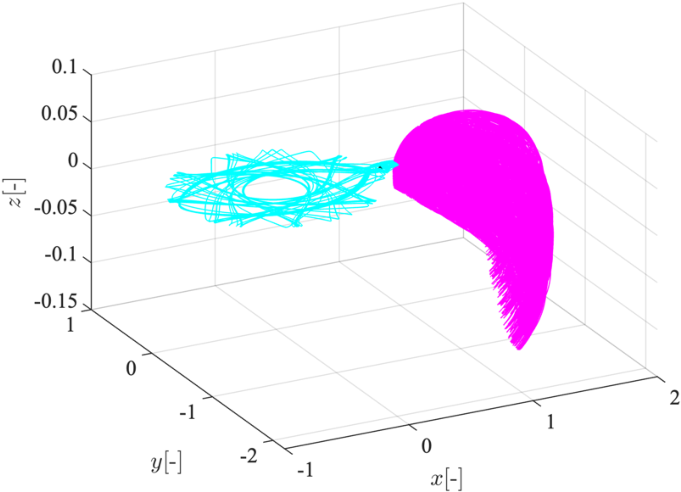
\includegraphics[width=50mm,clip]{fig/torus-lyap-manifold-global.pdf}
    \caption{Global view}
    \label{fig:sub-global}
  \end{subfigure}

  \vspace{5mm}

  \begin{subfigure}[b]{0.8\linewidth}
    \centering
    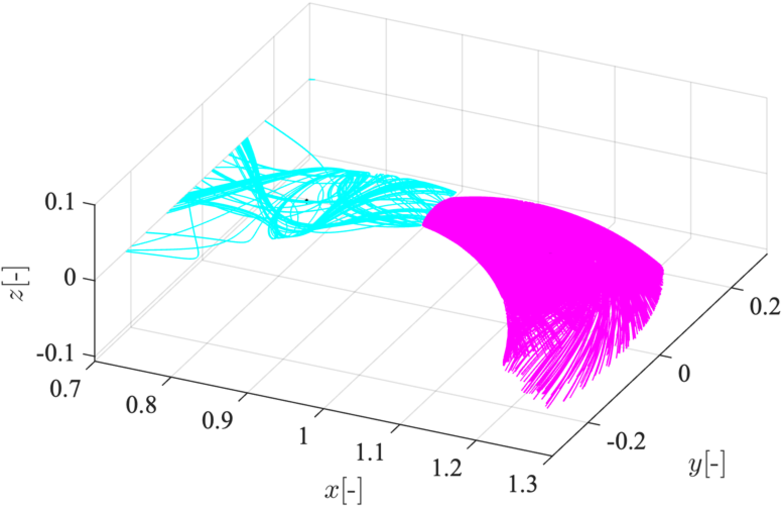
\includegraphics[width=50mm,clip]{fig/torus-lyap-manifold-zoomed.pdf}
    \caption{Zoomed-in view}
    \label{fig:sub-zoom}
  \end{subfigure}

  \caption{Propagation of the stable manifold from the Lyapunov orbit near $L_1$ (blue curve) and the unstable manifold from the quasi-periodic orbit near $L_2$ (red curve) to the connection plane at $x = 1-\mu$. The upper panel shows the global view, while the lower panel presents the zoomed view.}
  \label{torus lyapunov manifolds}
\end{figure}

For each manifold, interpolation functions $\gamma_1$ and $\gamma_2$ are constructed using two intrinsic parameters. In the case of the Lyapunov orbit, the parameters correspond to weights along the unstable directions($\theta_{11},\theta_{12}$), whereas for the quasi-periodic orbit they are given by the phase angles on the torus($\theta_{21},\theta_{22}$). These parameters uniquely determine points on the respective manifolds.

A Poincaré section is taken on an arbitrary plane($x = 1 - \mu$) to identify intersection points between the stable and unstable manifolds. Figs.\ref{torus lyapunov poincare} show the distributions of the stable and unstable manifolds on the Poincaré section in the $y-z-\dot{x}$ space, and the region with a high probability of intersection.

\begin{figure}[!t]
  \centering

  \begin{subfigure}[b]{0.8\linewidth}
    \centering
    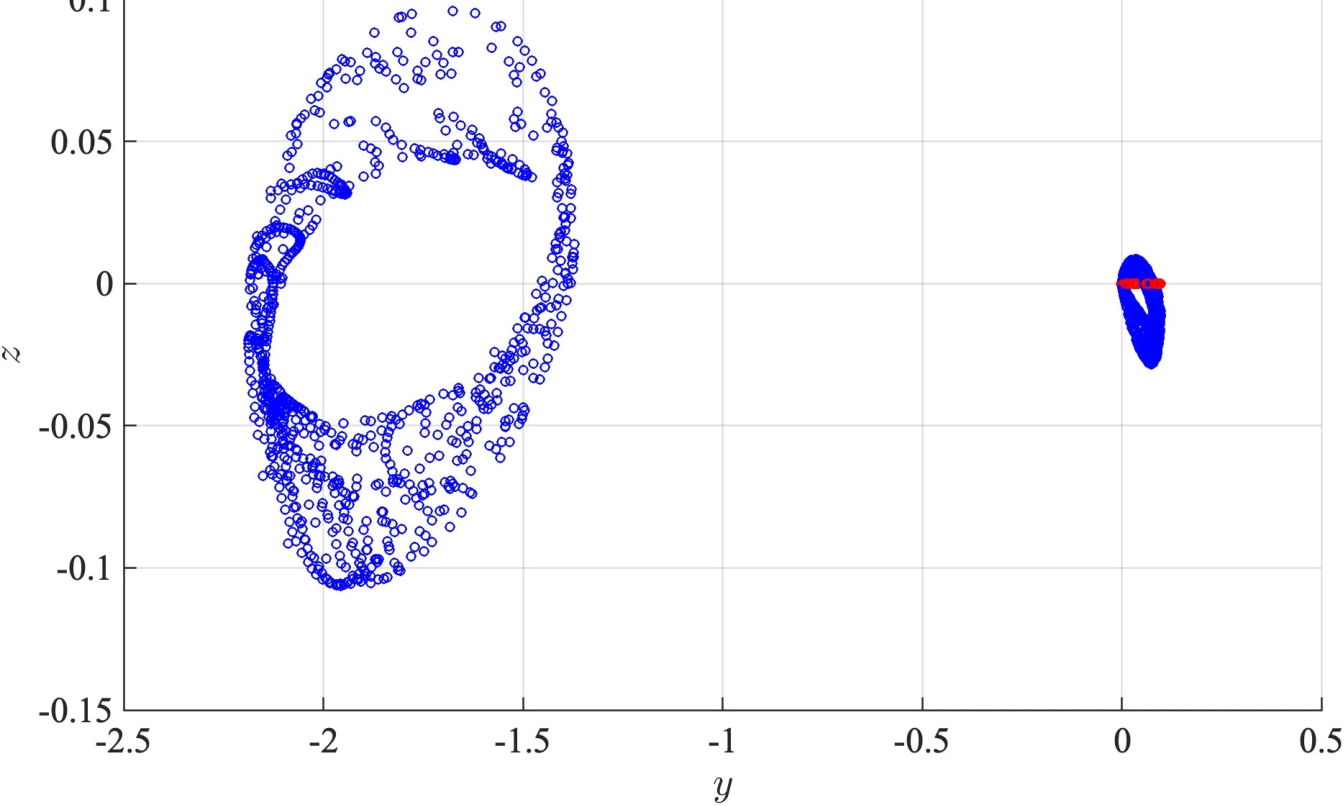
\includegraphics[width=50mm,clip]{fig/torus-lyap-poincare-global.pdf}
    \caption{Global view}
    \label{fig:sub-global}
  \end{subfigure}

  \vspace{5mm}

  \begin{subfigure}[b]{0.8\linewidth}
    \centering
    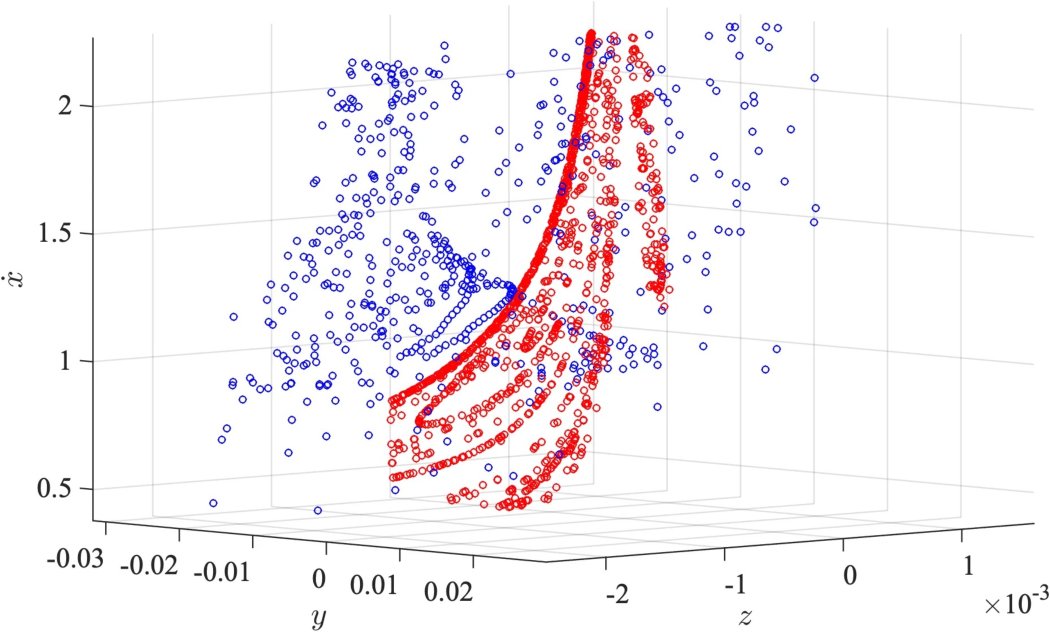
\includegraphics[width=50mm,clip]{fig/torus-lyap-poincare-zoomed.pdf}
    \caption{Zoomed-in view}
    \label{fig:sub-zoom}
  \end{subfigure}

  \caption{Distribution of stable and unstable manifolds on the Poincaré section($x = 1 - \mu$) in the $y-z-\dot{x}$ space.}
  \label{torus lyapunov poincare}
\end{figure}

However, intersection on this three-dimensional Poincaré section does not necessarily guarantee an intersection in the full six-dimensional phase space. As a preliminary assumption, intersections identified on the Poincaré section were initially regarded as indicative of intersections in six-dimensional space.

To resolve this issue, the selected candidate of the connection point was refined by utilizing interpolation functions constructed from the intrinsic parameters of the manifolds($\gamma_1,\gamma_2$). By imposing the Jacobi constant and Poincaré section conditions, the phase space dimension was reduced from six to four, and heteroclinic connections were thereby detected as manifold intersections in the reduced space. A candidate point obtained from the three-dimensional projection of the Poincaré section was refined by solving a nonlinear system derived from the evaluation function constructed with interpolation functions, thereby yielding a more accurate intersection of the manifolds. The nonlinear system was solved using Matlab's \texttt{fsolve}.

Based on the evaluation function, the associated trajectories were propagated, and a heteroclinic orbit connecting the in-plane Lyapunov orbit to the out-of-plane quasi-periodic orbit was successfully obtained. The global and zoomed-in views presented in Figs.\ref{torus lyapunov hetero} demonstrate this refined connection.

\begin{figure}[!t]
  \centering

  \begin{subfigure}[b]{0.8\linewidth}
    \centering
    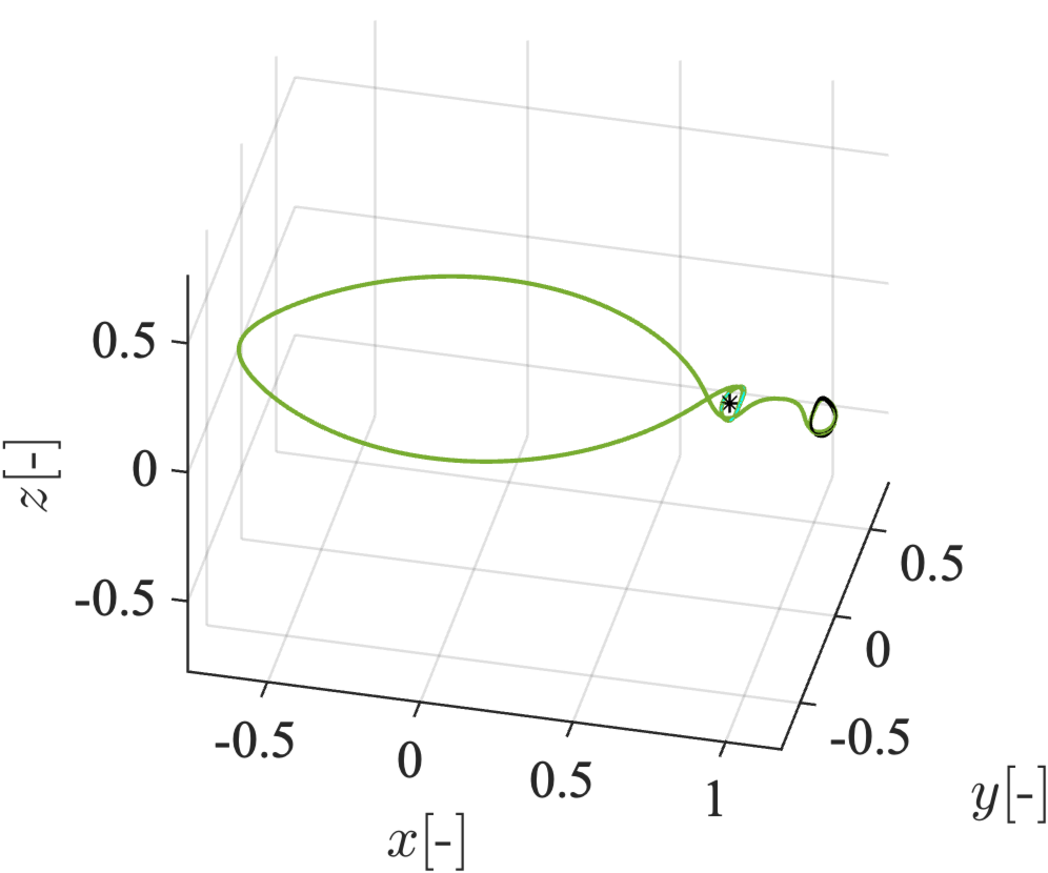
\includegraphics[width=50mm,clip]{fig/torus-lyap-hetero-glabal.pdf}
    \caption{Global view}
    \label{fig:sub-global}
  \end{subfigure}

  \vspace{5mm}

  \begin{subfigure}[b]{0.8\linewidth}
    \centering
    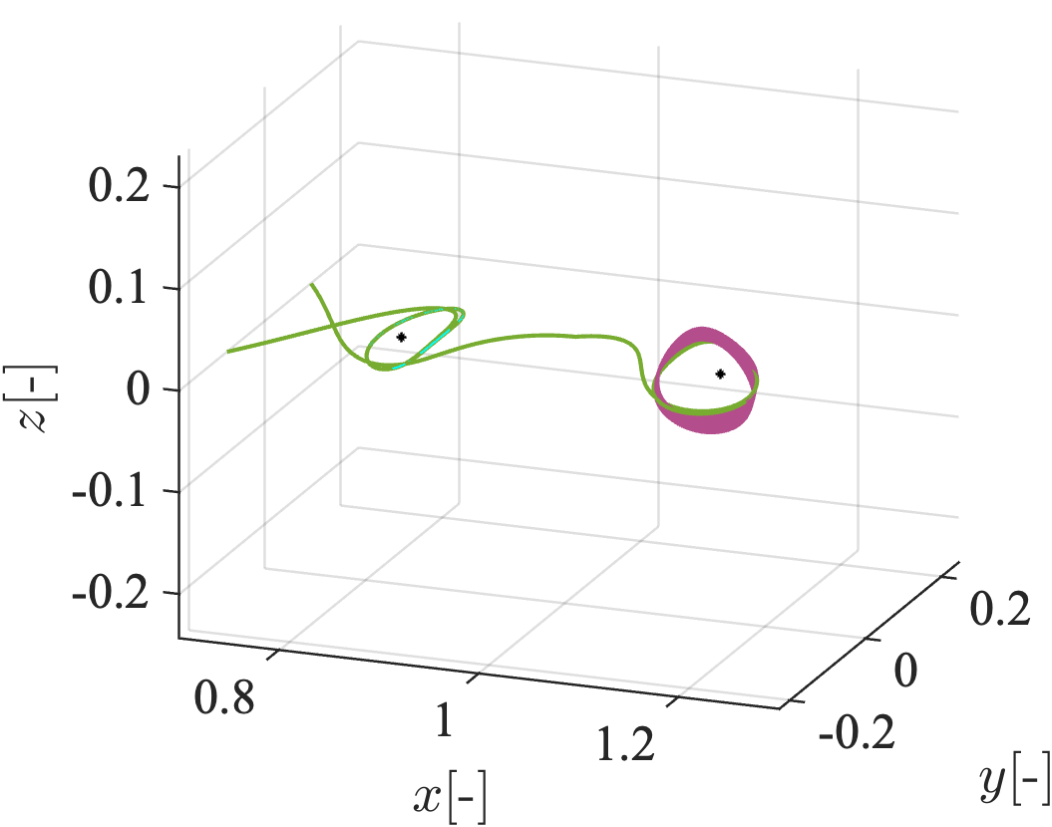
\includegraphics[width=50mm,clip]{fig/torus-lyap-hetero-zoomed.pdf}
    \caption{Zoomed-in view}
    \label{fig:sub-zoom}
  \end{subfigure}

  \caption{Computed heteroclinic connection between the Lyapunov orbit and the quasi-periodic orbit based on the selected intersection point.}
  \label{torus lyapunov hetero}
\end{figure}

\section{Conclusion}

In this study, heteroclinic connections between orbits of different geometric dimensions are investigated. By analyzing the connection dimensions between various combinations of orbit dimensions, the feasibility of such connections is assessed. The results indicate that heteroclinic connections are generally realizable in the six-dimensional phase space through the intersection of manifolds propagated from one-dimensional periodic orbits along two eigenvector directions and those associated with two-dimensional quasi-periodic orbits. Furthermore, by numerically propagating the stable and unstable manifolds and identifying intersection points using a Poincaré section, trajectories closely approximating heteroclinic connections between orbits of different dimensions are successfully computed.

\begin{appendices}
\section{Intersection Dimension Tables}
\label{Appendix_table}

This appendix shows the dimensional analysis of manifold intersections between various types of orbits in the planar and spatial circular restricted three-body problem (table~\ref{appendix_start}-~\ref{appendix_end}). Each table presents the dimension and co-dimension of the involved manifolds and computes the resulting intersection dimension $d_{int}$, providing insight into the existence of heteroclinic orbits between equilibrium points, periodic orbits, and quasi-periodic orbits.


\begin{table*}[htbp]
\centering
\caption{Dimensional analysis for manifolds between equilibrium points (Planar CR3BP).}
\label{appendix_start}
\begin{tabular}{lccccl}
\bhline{0.8pt}
& Manifold of equilibrium point & Manifold of equilibrium & & \\
\hline
Dimension ($m$) & 1 & 1 & 3 & Dimension, phase space ($n$) \\
Co-dimension ($l$) & 2 & 2 & 4 & Co-dimension, intersection \\
& & & -1 & Dimension, intersection ($d_{int}$) \\ \bhline{0.8pt}
\end{tabular}
\end{table*}

\vspace{1em}

\begin{table*}[htbp]
\centering
\caption{Dimensional analysis for manifolds between equilibrium point and periodic orbit (Planar CR3BP).}
\begin{tabular}{lccccl}
\bhline{0.8pt}
& Manifold of equilibrium point & Manifold of periodic orbit & & \\
\hline
Dimension ($m$) & 1 & 2 & 3 & Dimension, phase space ($n$) \\
Co-dimension ($l$) & 2 & 1 & 3 & Co-dimension, intersection \\
& & & 0 & Dimension, intersection ($d_{int}$) \\ \bhline{0.8pt}
\end{tabular}
\end{table*}

\vspace{1em}

\begin{table*}[htbp]
\centering
\caption{Dimensional analysis for manifolds between periodic orbits (Planar CR3BP).}
\begin{tabular}{lccccl}
\bhline{0.8pt}
& Manifold of periodic orbit & Manifold of periodic orbit & & \\
\hline
Dimension ($m$) & 2 & 2 & 3 & Dimension, phase space ($n$) \\
Co-dimension ($l$) & 1 & 1 & 2 & Co-dimension, intersection \\
& & & 1 & Dimension, intersection ($d_{int}$) \\ \bhline{0.8pt}
\end{tabular}
\end{table*}

\vspace{1em}

\begin{table*}[htbp]
\centering
\caption{Dimensional analysis for manifolds between equilibrium points  (Spatial CR3BP).}
\begin{tabular}{lccccl}
\bhline{0.8pt}
& Manifold of equilibrium point & Manifold of equilibrium point & & \\
\hline
Dimension ($m$) & 1 & 1 & 5 & Dimension, phase space ($n$) \\
Co-dimension ($l$) & 4 & 4 & 8 & Co-dimension, intersection \\
& & & -3 & Dimension, intersection ($d_{int}$) \\ \bhline{0.8pt}
\end{tabular}
\end{table*}

\vspace{1em}

\begin{table*}[htbp]
\centering
\caption{Dimensional analysis for manifolds between equilibrium point and periodic orbit  (Spatial CR3BP).}
\begin{tabular}{lccccl}
\bhline{0.8pt}
& Manifold of equilibrium point & Manifold of periodic orbit & & \\
\hline
Dimension ($m$) & 1 & 2 & 5 & Dimension, phase space ($n$) \\
Co-dimension ($l$) & 4 & 3 & 7 & Co-dimension, intersection \\
& & & -2 & Dimension, intersection ($d_{int}$) \\ \bhline{0.8pt}
\end{tabular}
\end{table*}

\vspace{1em}

\begin{table*}[htbp]
\centering
\caption{Dimensional analysis for manifolds between equilibrium point and periodic orbit  (Spatial CR3BP).}
\begin{tabular}{lccccl}
\bhline{0.8pt}
& Manifold of equilibrium point & Manifold of periodic orbit & & \\
\hline
Dimension ($m$) & 1 & 2 & 5 & Dimension, phase space ($n$) \\
Co-dimension ($l$) & 4 & 3 & 7 & Co-dimension, intersection \\
& & & -2 & Dimension, intersection ($d_{int}$) \\ \bhline{0.8pt}
\end{tabular}
\end{table*}

\vspace{1em}

\begin{table*}[htbp]
\centering
\caption{Dimensional analysis for manifolds between equilibrium point and periodic orbit with two eigenvector direction  (Spatial CR3BP).}
\begin{tabular}{lccccl}
\bhline{0.8pt}
& Manifold of equilibrium point & Manifold of periodic orbit (2-dir) & & \\
\hline
Dimension ($m$) & 1 & 3 & 5 & Dimension, phase space ($n$) \\
Co-dimension ($l$) & 4 & 2 & 6 & Co-dimension, intersection \\
& & & -1 & Dimension, intersection ($d_{int}$) \\ \bhline{0.8pt}
\end{tabular}
\end{table*}

\vspace{1em}

\begin{table*}[htbp]
\centering
\caption{Dimensional analysis for manifolds between equilibrium point and quasi-periodic orbit  (Spatial CR3BP).}
\begin{tabular}{lccccl}
\bhline{0.8pt}
& Manifold of equilibrium point & Manifold of quasi-periodic orbit & & \\
\hline
Dimension ($m$) & 1 & 3 & 5 & Dimension, phase space ($n$) \\
Co-dimension ($l$) & 4 & 2 & 6 & Co-dimension, intersection \\
& & & -1 & Dimension, intersection ($d_{int}$) \\ \bhline{0.8pt}
\end{tabular}
\end{table*}

\vspace{1em}

\begin{table*}[htbp]
\centering
\caption{Dimensional analysis for manifolds between periodic orbits  (Spatial CR3BP).}
\begin{tabular}{lccccl}
\bhline{0.8pt}
& Manifold of periodic orbit & Manifold of periodic orbit & & \\
\hline
Dimension ($m$) & 2 & 2 & 5 & Dimension, phase space ($n$) \\
Co-dimension ($l$) & 3 & 3 & 6 & Co-dimension, intersection \\
& & & -1 & Dimension, intersection ($d_{int}$) \\ \bhline{0.8pt}
\end{tabular}
\end{table*}

\vspace{1em}

\begin{table*}[htbp]
\centering
\caption{Dimensional analysis for manifolds between periodic orbit and periodic orbit with two eigenvector direction  (Spatial CR3BP).}
\begin{tabular}{lccccl}
\bhline{0.8pt}
& Manifold of periodic orbit & Manifold of periodic orbit (2-dir) & & \\
\hline
Dimension ($m$) & 2 & 3 & 5 & Dimension, phase space ($n$) \\
Co-dimension ($l$) & 3 & 2 & 5 & Co-dimension, intersection \\
& & & 0 & Dimension, intersection ($d_{int}$) \\ \bhline{0.8pt}
\end{tabular}
\end{table*}

\vspace{1em}

\begin{table*}[htbp]
\centering
\caption{Dimensional analysis for manifolds between periodic orbit and quasi-periodic orbit (Spatial CR3BP).}
\begin{tabular}{lccccl}
\bhline{0.8pt}
& Manifold of periodic orbit & Manifold of quasi-periodic orbit & & \\
\hline
Dimension ($m$) & 2 & 3 & 5 & Dimension, phase space ($n$) \\
Co-dimension ($l$) & 3 & 2 & 5 & Co-dimension, intersection \\
& & & 0 & Dimension, intersection ($d_{int}$) \\ \bhline{0.8pt}
\end{tabular}
\end{table*}

\vspace{1em}

\begin{table*}[htbp]
\centering
\caption{Dimensional analysis for manifolds between periodic orbits with two eigenvector direction  (Spatial CR3BP).}
\begin{tabular}{lccccl}
\bhline{0.8pt}
& Manifold of periodic orbit (2-dir) & Manifold of periodic orbit (2-dir) & & \\
\hline
Dimension ($m$) & 3 & 3 & 5 & Dimension, phase space ($n$) \\
Co-dimension ($l$) & 2 & 2 & 4 & Co-dimension, intersection \\
& & & 1 & Dimension, intersection ($d_{int}$) \\ \bhline{0.8pt}
\end{tabular}
\end{table*}

\vspace{1em}

\begin{table*}[htbp]
\centering
\caption{Dimensional analysis for manifolds between periodic orbit with two eigenvector direction and quasi-periodic orbit  (Spatial CR3BP).}
\begin{tabular}{lccccl}
\bhline{0.8pt}
& Manifold of periodic orbit (2-dir) & Manifold of quasi-periodic orbit & & \\
\hline
Dimension ($m$) & 3 & 3 & 5 & Dimension, phase space ($n$) \\
Co-dimension ($l$) & 2 & 2 & 4 & Co-dimension, intersection \\
& & & 1 & Dimension, intersection ($d_{int}$) \\ \bhline{0.8pt}
\end{tabular}
\end{table*}

\vspace{1em}

\begin{table*}[htbp]
\centering
\caption{Dimensional analysis for manifolds between quasi-periodic orbits (Spatial CR3BP).}
\label{appendix_end}
\begin{tabular}{lccccl}
\bhline{0.8pt}
& Manifold of quasi-periodic orbit & Manifold of quasi-periodic orbit & & \\
\hline
Dimension ($m$) & 3 & 3 & 5 & Dimension, phase space ($n$) \\
Co-dimension ($l$) & 2 & 2 & 4 & Co-dimension, intersection \\
& & & 1 & Dimension, intersection ($d_{int}$) \\ \bhline{0.8pt}
\end{tabular}
\end{table*}

\end{appendices}

\bibliographystyle{plain}  % または abbrv, unsrt, ieeetr, etc.

\bibliography{reference}  

\end{document}
